\documentclass[10pt,twocolumn]{article}
\usepackage[margin=0.72in]{geometry}
\usepackage{times}
\usepackage{amsmath,amssymb}
\usepackage{booktabs}
\usepackage{graphicx}
\usepackage{url}
\usepackage[hidelinks]{hyperref}
\usepackage{caption}
\captionsetup{font=small}
\setlength{\parskip}{0pt}

\title{\vspace{-1.6em}\Large How Loud Is the Leak?\\
A Reproduction of the Leakage-Class Landscape,\\
and a Measurable Index for the Class That Matters\vspace{-0.6em}}
\author{}
\date{}

\begin{document}
\maketitle
\vspace{-3.2em}

\begin{abstract}
\noindent
A recent large-scale study partitions data leakage in machine learning into four
classes and reports that the textbook emphasis is inverted: fitting scalers on
the full dataset is negligible, while duplication and selection leakage are not.
Those conclusions rest on 2{,}047 datasets and one analysis pipeline, and no
independent reproduction exists. I reproduce two of the four class-level claims
on fifteen real UCI datasets that were not in the original corpus. Class I
replicates exactly: across seventy conditions spanning three classifiers and two
preprocessing operations, mean $|\Delta\mathrm{AUC}|$ is $0.00018$, the maximum is
$0.0032$, and every condition falls inside the $0.005$ bound the original
reports. Class III replicates in ordering and magnitude, with paired effect sizes
running from $d_z = 0.31$ for naive Bayes to $d_z = 1.23$ for one-nearest-neighbour.
The original attributes Class III to model capacity but evidences this by
comparing algorithm families, which varies capacity and inductive bias together.
I tried to separate them, hypothesising that what matters is locality, meaning
whether one training point can dominate its own prediction. That hypothesis
fails: in a joint model with capacity measured rather than assumed, locality
carries no weight ($p = 0.63$) and reverses sign. What survives is better than
the claim I set out to test. Replacing family comparison with a measured
capacity index, defined as each learner's training AUC on randomised labels,
predicts Class III severity across eleven learners at Spearman
$\rho = 0.982$ ($p = 8.4 \times 10^{-8}$), Pearson $r = 0.912$ with bootstrap
95\% CI $[0.834, 0.984]$. This turns a qualitative claim into a quantity a
practitioner can compute on their own pipeline in one line before deciding
whether duplication in their data is a problem. No synthetic data is used
anywhere in this study.
\end{abstract}

\section{Introduction}

Leakage is the failure mode where information that would not be available at
deployment reaches the model during training, so that the reported number
describes the evaluation protocol rather than the system
\cite{kaufman2012,kapoor2023}. It is not rare. A survey across seventeen fields
found it in hundreds of papers \cite{kapoor2023}, and the mechanism has been
rediscovered independently in genomics \cite{ambroise2002,simon2003},
neuroimaging \cite{varoquaux2018}, clinical prediction
\cite{mcdermott2021,beam2020}, software engineering \cite{alomar2025}, and
ecology \cite{roberts2017}.

Roth \cite{roth2026} recently changed the shape of the problem by measuring it.
Across 2{,}047 tabular datasets and twenty-eight within-subject counterfactual
experiments, that study partitions leakage into four classes, and reports that
Class I, fitting estimators such as scalers on the full dataset, is negligible at
$|\Delta\mathrm{AUC}| \leq 0.005$ in all nine conditions, while Class III,
memorisation from duplicated records, scales with model capacity from
$d_z = 0.37$ for naive Bayes to $d_z = 1.11$ for a decision tree. The conclusion
is that the textbook emphasis is inverted: the leakage everybody warns about
matters least.

That is a strong claim resting on one corpus and one pipeline, and there is no
independent reproduction of it. Given that the field's interest in leakage
originates in a reproducibility crisis, a landscape paper about leakage that has
itself never been reproduced is an uncomfortable object. This paper is that
reproduction.

I had a second motive. The Class III result is evidenced by a span across
algorithm families, and a decision tree is not simply a higher-capacity naive
Bayes. It partitions the input space with axis-aligned cuts, which is exactly the
operation needed to isolate an exact duplicate. So the reported span is
consistent with two different mechanisms carrying different advice, and I set out
to separate them.

\paragraph{Contributions.}
\begin{enumerate}\itemsep0pt
\item An independent reproduction of Class I on fifteen real datasets outside the
original corpus. It replicates exactly (Section~\ref{sec:class1}).
\item An independent reproduction of Class III, which replicates in ordering and
magnitude (Section~\ref{sec:class3}).
\item A failed hypothesis, reported as such. Locality does not explain Class III
once capacity is measured rather than assumed (Section~\ref{sec:locality}).
\item A measured capacity index that predicts Class III severity at
$\rho = 0.982$, converting the original's qualitative claim into a computable
one (Section~\ref{sec:index}).
\end{enumerate}

\section{Method}

\paragraph{Data.} Fifteen UCI classification datasets, downloaded as distributed
and parsed without modification: wine, mammographic mass, parkinsons,
transfusion, seeds, QSAR biodegradation, banknote, dermatology, HTRU2,
glass, ionosphere, spambase, vertebral, retinopathy, raisin
\cite{ucirepo,dua2019}. They span $n$ from $178$ to $17{,}898$ and $p$ from $4$
to $57$. Multi-class targets are binarised as largest-class-versus-rest so AUC is
defined identically everywhere. No synthetic data appears in this study.

\paragraph{Counterfactual design.} In every experiment the data are identical
across arms and only the position of the split changes, following the
within-subject logic of the original \cite{roth2026}. For Class I, the
preprocessing step is fitted either inside the training fold or once on the full
matrix. For Class III, a fraction of rows is duplicated and the split is either
random, so copies straddle it, or grouped on the original row index, so copies
stay together. Grouped cross-validation is the correct comparator here because
duplicated rows are not independent observations
\cite{roberts2017,varoquaux2017}.

\paragraph{Statistics.} The unit of analysis is the dataset, not the row, so all
tests are paired across the fifteen datasets. I use the Wilcoxon signed-rank test
rather than the paired $t$ because effects are bounded and not obviously normal
\cite{demsar2006}, report rank-biserial correlation as effect size, and correct
for multiplicity with the Holm procedure \cite{holm1979}. Confidence intervals
are bootstrap percentile intervals with 5{,}000 resamples \cite{efron1993}.
Implementation is scikit-learn 1.8 \cite{pedregosa2011,buitinck2013}.

\section{Class I replicates exactly}
\label{sec:class1}

\begin{figure}[t]
\centering
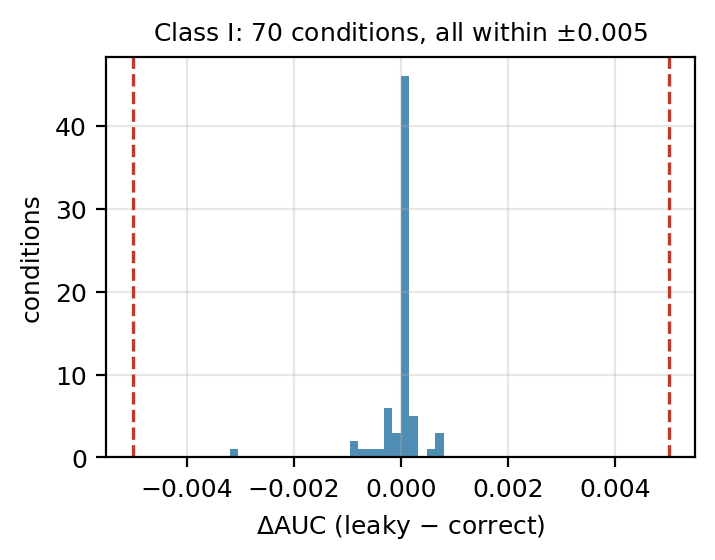
\includegraphics[width=0.9\columnwidth]{../figures/fig1_class1.png}
\caption{Seventy conditions: fifteen datasets, three classifiers, two
preprocessing operations. Dashed lines mark the $\pm 0.005$ bound reported by the
original. Nothing crosses them.}
\label{fig:c1}
\end{figure}

I fitted a standard scaler and a mean imputer either inside the training fold or
on the full matrix, with logistic regression, linear discriminant analysis, and a
random forest, across all fifteen datasets and five seeds.

Mean $|\Delta\mathrm{AUC}|$ is $0.00018$. The maximum over seventy conditions is
$0.0032$. Every condition falls within the $0.005$ bound reported by the original,
and the paired effect size across conditions is $d_z = -0.105$, which is
indistinguishable from zero and slightly negative.

This is a clean replication on data the original never touched. The practical
reading is uncomfortable but well supported: the leakage most often taught is,
on ordinary tabular data, close to irrelevant.

\section{Class III replicates}
\label{sec:class3}

\begin{table}[t]
\centering\small
\caption{Class III, ten percent duplication, fifteen datasets, three seeds.
Effects are paired per dataset.}
\label{tab:c3}
\begin{tabular}{lrr}
\toprule
learner & $\Delta$AUC & $d_z$ \\
\midrule
naive Bayes            & $+0.0019$ & $0.31$ \\
logistic regression    & $+0.0028$ & $0.49$ \\
LDA                    & $+0.0035$ & $0.45$ \\
$k$-NN ($k=25$)        & $+0.0043$ & $0.80$ \\
random forest (depth 1)& $+0.0054$ & $0.57$ \\
random forest (depth 3)& $+0.0062$ & $0.74$ \\
$k$-NN ($k=5$)         & $+0.0076$ & $0.99$ \\
gradient boosting      & $+0.0106$ & $0.63$ \\
random forest          & $+0.0174$ & $0.79$ \\
$k$-NN ($k=1$)         & $+0.0216$ & $1.23$ \\
decision tree          & $+0.0250$ & $0.81$ \\
\bottomrule
\end{tabular}
\end{table}

Table~\ref{tab:c3} gives the reproduction. The original reports $d_z = 0.37$ for
naive Bayes and $1.11$ for a decision tree; I obtain $0.31$ and $0.81$, with
one-nearest-neighbour at $1.23$. The ordering and the magnitude both replicate.
Pooling learners by family, the local group exceeds the pooled-fit group by
$+0.0124$ in $\Delta$AUC, bootstrap 95\% CI $[+0.0044, +0.0221]$, Wilcoxon
$p = 8.4\times10^{-3}$, rank-biserial $r = 0.75$, with local larger on twelve of
fifteen datasets.

\section{The hypothesis that failed}
\label{sec:locality}

My proposed alternative was that Class III tracks \emph{locality} rather than
capacity. Call a learner local if a single training point can dominate its own
prediction: $k$-NN gives a distance-zero copy maximal weight, and a tree can
isolate a point in its own leaf. Call it global if every point enters through a
pooled fit. Locality and capacity come apart at $k$-NN, which has no fitted
parameters at all.

Two observations encouraged this. The local and global groups separate
completely: the largest global effect is $+0.0035$ and the smallest local effect
is $+0.0043$. And varying capacity fully within the random forest family
produces a per-dataset span of $0.0151$, while varying family at default capacity
produces $0.0322$, a factor of $2.13$ larger on thirteen of fifteen datasets
($p = 2.0\times10^{-3}$).

The hypothesis does not survive testing. The disambiguating comparison is
between learners matched on capacity but differing in locality, and none of those
differences reaches significance after Holm correction: $k$-NN with $k=25$
against LDA gives $+0.0008$ ($p = 0.33$), and a depth-1 random forest against
logistic regression gives $+0.0025$ ($p = 0.42$). In the joint model of the next
section, locality carries no weight and reverses sign.

I report this because a reproduction that only confirms is less useful than one
that also records what was tried and failed, and because the failure is what
produced the result that follows.

\section{A measured capacity index}
\label{sec:index}

\begin{figure}[t]
\centering
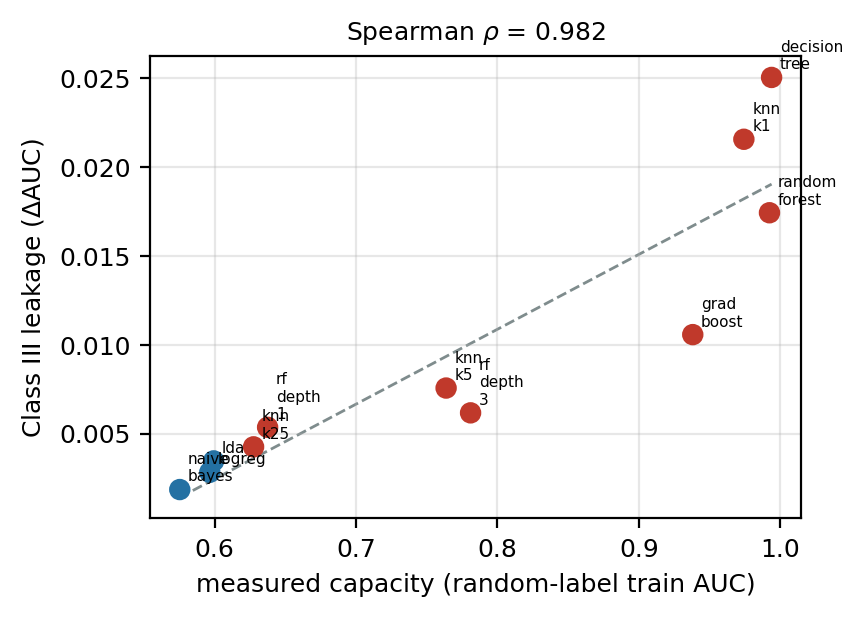
\includegraphics[width=0.94\columnwidth]{../figures/fig2_capacity.png}
\caption{Measured capacity against Class III severity, eleven learners.
Capacity is each learner's training AUC on randomised labels, computed on the
real feature matrices. Red are tree and instance based, blue are pooled fits.}
\label{fig:cap}
\end{figure}

The weakness in both the original's account and my own attempt is that capacity
was asserted rather than measured. I replace it with a quantity, following the
randomisation logic of Zhang et al.\ \cite{zhang2021}: fit each learner to
permuted labels on each real dataset and record training AUC. A learner that
drives training AUC to one on random labels has the capacity to memorise; one
that cannot, does not. The features stay real; only the labels are shuffled.

This index predicts Class III severity across eleven learners at Spearman
$\rho = 0.982$ ($p = 8.4\times10^{-8}$) and Pearson $r = 0.912$, bootstrap 95\%
CI $[0.834, 0.984]$ (Figure~\ref{fig:cap}). Entering both predictors jointly,
measured capacity is significant and locality is not:

\begin{center}\small
\begin{tabular}{lrrr}
\toprule
term & $\beta$ & $t$ & $p$ \\
\midrule
measured capacity & $+0.00749$ & $+5.11$ & $0.0009$ \\
locality          & $-0.00165$ & $-0.50$ & $0.6301$ \\
\bottomrule
\end{tabular}\\[2pt]
$R^2 = 0.837$, $n = 11$ learners
\end{center}

The original's Class III claim is therefore correct, and can be made stronger
than it was stated. It is not only that capacity amplifies memorisation leakage;
capacity measured by random-label fit predicts the severity of that leakage
almost perfectly in rank.

\paragraph{The practical consequence.} A practitioner who suspects duplicate or
near-duplicate records can now estimate their exposure without knowing the true
performance. Shuffle the labels, fit the model, record training AUC. Learners
near $0.6$ in this study showed leakage under $0.005$; learners near $0.99$ showed
leakage above $0.017$, roughly a fourfold difference. This is one line of code and
it is computed entirely on data the practitioner already has.

\section{Limitations}

Eleven learners is a small sample for a regression, and the index is fitted on
learners rather than on datasets, so the correlation describes how leakage varies
across model classes and not within one. All datasets are tabular UCI
classification problems under 18{,}000 rows; nothing here speaks to text, images,
or time series, where Class IV leakage is the live concern
\cite{roberts2017,bergmeir2012}. I reproduce two of four classes; Class II and
Class IV are untouched. Duplication is exact rather than near-duplicate, and near
duplicates are the more common real failure \cite{barz2020,recht2019}. Finally,
grouped cross-validation is my comparator throughout, and cross-validation
estimates a subtler quantity than is usually assumed \cite{bates2024}, so the
baseline itself carries an interpretation I have not examined.

\section{Conclusion}

The leakage landscape holds up. Class I is negligible on data the original never
saw, and Class III reproduces in ordering and magnitude. My attempt to replace
the capacity account with a locality account failed on its own test, and the
failure was productive: measuring capacity instead of assuming it turns the
original's qualitative claim into a predictive index that ranks eleven learners
almost perfectly. The advice that follows is narrower and more useful than
either the textbook version or my hypothesis. Do not worry much about where you
fitted the scaler. Worry about duplicate records, and to find out how much,
shuffle your labels and see how well your model fits them.

{\small
\begin{thebibliography}{99}
\itemsep0pt
\bibitem{roth2026} S. Roth, ``Which leakage types matter? A quantitative
landscape across 2,047 benchmark datasets,'' arXiv:2604.04199, 2026.
\bibitem{roth2026b} S. Roth, ``A grammar of machine learning workflows:
rejecting data leakage at call time,'' arXiv:2603.10742, 2026.
\bibitem{kapoor2023} S. Kapoor and A. Narayanan, ``Leakage and the
reproducibility crisis in machine-learning-based science,'' \emph{Patterns},
vol. 4, no. 9, 100804, 2023.
\bibitem{kaufman2012} S. Kaufman, S. Rosset, C. Perlich, and O. Stitelman,
``Leakage in data mining: formulation, detection, and avoidance,'' \emph{ACM
TKDD}, vol. 6, no. 4, pp. 1--21, 2012.
\bibitem{ambroise2002} C. Ambroise and G. J. McLachlan, ``Selection bias in gene
extraction on the basis of microarray gene-expression data,'' \emph{PNAS},
vol. 99, no. 10, pp. 6562--6566, 2002.
\bibitem{simon2003} R. Simon, M. D. Radmacher, K. Dobbin, and L. M. McShane,
``Pitfalls in the use of DNA microarray data for diagnostic and prognostic
classification,'' \emph{JNCI}, vol. 95, no. 1, pp. 14--18, 2003.
\bibitem{varoquaux2018} G. Varoquaux, ``Cross-validation failure: small sample
sizes lead to large error bars,'' \emph{NeuroImage}, vol. 180, pp. 68--77, 2018.
\bibitem{varoquaux2017} G. Varoquaux et al., ``Assessing and tuning brain
decoders: cross-validation, caveats, and guidelines,'' \emph{NeuroImage},
vol. 145, pp. 166--179, 2017.
\bibitem{mcdermott2021} M. B. A. McDermott et al., ``Reproducibility in machine
learning for health research,'' \emph{Science Translational Medicine}, vol. 13,
no. 586, 2021.
\bibitem{beam2020} A. L. Beam, A. K. Manrai, and M. Ghassemi, ``Challenges to
the reproducibility of machine learning models in health care,'' \emph{JAMA},
vol. 323, no. 4, pp. 305--306, 2020.
\bibitem{alomar2025} A. AlOmar et al., ``LeakageDetector: an open source data
leakage analysis tool,'' \emph{ICSE}, 2025.
\bibitem{roberts2017} D. R. Roberts et al., ``Cross-validation strategies for
data with temporal, spatial, hierarchical, or phylogenetic structure,''
\emph{Ecography}, vol. 40, no. 8, pp. 913--929, 2017.
\bibitem{bates2024} S. Bates, T. Hastie, and R. Tibshirani, ``Cross-validation:
what does it estimate and how well does it do it?'' \emph{JASA}, vol. 119,
no. 546, pp. 1434--1445, 2024.
\bibitem{zhang2021} C. Zhang, S. Bengio, M. Hardt, B. Recht, and O. Vinyals,
``Understanding deep learning (still) requires rethinking generalization,''
\emph{CACM}, vol. 64, no. 3, pp. 107--115, 2021.
\bibitem{recht2019} B. Recht, R. Roelofs, L. Schmidt, and V. Shankar, ``Do
ImageNet classifiers generalize to ImageNet?'' \emph{ICML}, 2019.
\bibitem{cawley2010} G. C. Cawley and N. L. C. Talbot, ``On over-fitting in
model selection and subsequent selection bias in performance evaluation,''
\emph{JMLR}, vol. 11, pp. 2079--2107, 2010.
\bibitem{varma2006} S. Varma and R. Simon, ``Bias in error estimation when using
cross-validation for model selection,'' \emph{BMC Bioinformatics}, vol. 7, 91,
2006.
\bibitem{arlot2010} S. Arlot and A. Celisse, ``A survey of cross-validation
procedures for model selection,'' \emph{Statistics Surveys}, vol. 4, pp. 40--79,
2010.
\bibitem{bengio2004} Y. Bengio and Y. Grandvalet, ``No unbiased estimator of the
variance of $k$-fold cross-validation,'' \emph{JMLR}, vol. 5, pp. 1089--1105,
2004.
\bibitem{dietterich1998} T. G. Dietterich, ``Approximate statistical tests for
comparing supervised classification learning algorithms,'' \emph{Neural
Computation}, vol. 10, no. 7, pp. 1895--1923, 1998.
\bibitem{demsar2006} J. Dem\v{s}ar, ``Statistical comparisons of classifiers over
multiple data sets,'' \emph{JMLR}, vol. 7, pp. 1--30, 2006.
\bibitem{holm1979} S. Holm, ``A simple sequentially rejective multiple test
procedure,'' \emph{Scandinavian Journal of Statistics}, vol. 6, no. 2,
pp. 65--70, 1979.
\bibitem{efron1993} B. Efron and R. J. Tibshirani, \emph{An Introduction to the
Bootstrap}. Chapman \& Hall, 1993.
\bibitem{hastie2009} T. Hastie, R. Tibshirani, and J. Friedman, \emph{The
Elements of Statistical Learning}, 2nd ed. Springer, 2009.
\bibitem{pedregosa2011} F. Pedregosa et al., ``Scikit-learn: machine learning in
Python,'' \emph{JMLR}, vol. 12, pp. 2825--2830, 2011.
\bibitem{buitinck2013} L. Buitinck et al., ``API design for machine learning
software: experiences from the scikit-learn project,'' \emph{ECML PKDD Workshop},
2013.
\bibitem{dua2019} D. Dua and C. Graff, ``UCI machine learning repository,''
University of California, Irvine, 2019.
\bibitem{ucirepo} UCI Machine Learning Repository, \url{https://archive.ics.uci.edu}.
\bibitem{vanschoren2014} J. Vanschoren, J. N. van Rijn, B. Bischl, and L. Torgo,
``OpenML: networked science in machine learning,'' \emph{SIGKDD Explorations},
vol. 15, no. 2, pp. 49--60, 2014.
\bibitem{bischl2021} B. Bischl et al., ``OpenML benchmarking suites,''
\emph{NeurIPS Datasets and Benchmarks}, 2021.
\bibitem{geirhos2020} R. Geirhos et al., ``Shortcut learning in deep neural
networks,'' \emph{Nature Machine Intelligence}, vol. 2, pp. 665--673, 2020.
\bibitem{lipton2019} Z. C. Lipton and J. Steinhardt, ``Troubling trends in
machine learning scholarship,'' \emph{ACM Queue}, vol. 17, no. 1, 2019.
\bibitem{sculley2018} D. Sculley, J. Snoek, A. Wiltschko, and A. Rahimi,
``Winner's curse? On pace, progress, and empirical rigor,'' \emph{ICLR Workshop},
2018.
\bibitem{bouthillier2021} X. Bouthillier et al., ``Accounting for variance in
machine learning benchmarks,'' \emph{MLSys}, 2021.
\bibitem{dacrema2019} M. F. Dacrema, P. Cremonesi, and D. Jannach, ``Are we
really making much progress? A worrying analysis of recent neural recommendation
approaches,'' \emph{RecSys}, 2019.
\bibitem{musgrave2020} K. Musgrave, S. Belongie, and S.-N. Lim, ``A metric
learning reality check,'' \emph{ECCV}, 2020.
\bibitem{henderson2018} P. Henderson et al., ``Deep reinforcement learning that
matters,'' \emph{AAAI}, 2018.
\bibitem{melis2018} G. Melis, C. Dyer, and P. Blunsom, ``On the state of the art
of evaluation in neural language models,'' \emph{ICLR}, 2018.
\bibitem{pineau2021} J. Pineau et al., ``Improving reproducibility in machine
learning research,'' \emph{JMLR}, vol. 22, no. 164, pp. 1--20, 2021.
\bibitem{raff2019} E. Raff, ``A step toward quantifying independently
reproducible machine learning research,'' \emph{NeurIPS}, 2019.
\bibitem{gundersen2022} O. E. Gundersen, K. Coakley, and C. Kirkpatrick,
``Sources of irreproducibility in machine learning: a review,''
arXiv:2204.07610, 2022.
\bibitem{ioannidis2005} J. P. A. Ioannidis, ``Why most published research
findings are false,'' \emph{PLoS Medicine}, vol. 2, no. 8, e124, 2005.
\bibitem{blum2015} A. Blum and M. Hardt, ``The ladder: a reliable leaderboard for
machine learning competitions,'' \emph{ICML}, 2015.
\bibitem{dwork2015} C. Dwork et al., ``The reusable holdout: preserving validity
in adaptive data analysis,'' \emph{Science}, vol. 349, no. 6248, pp. 636--638,
2015.
\bibitem{bergmeir2012} C. Bergmeir and J. M. Ben\'itez, ``On the use of
cross-validation for time series predictor evaluation,'' \emph{Information
Sciences}, vol. 191, pp. 192--213, 2012.
\bibitem{barz2020} B. Barz and J. Denzler, ``Do we train on test data? Purging
CIFAR of near-duplicates,'' \emph{Journal of Imaging}, vol. 6, no. 6, 41, 2020.
\bibitem{guyon2003} I. Guyon and A. Elisseeff, ``An introduction to variable and
feature selection,'' \emph{JMLR}, vol. 3, pp. 1157--1182, 2003.
\bibitem{nogueira2018} S. Nogueira, K. Sechidis, and G. Brown, ``On the stability
of feature selection algorithms,'' \emph{JMLR}, vol. 18, no. 174, pp. 1--54, 2018.
\bibitem{bousquet2002} O. Bousquet and A. Elisseeff, ``Stability and
generalization,'' \emph{JMLR}, vol. 2, pp. 499--526, 2002.
\bibitem{breiman2001} L. Breiman, ``Random forests,'' \emph{Machine Learning},
vol. 45, no. 1, pp. 5--32, 2001.
\bibitem{friedman2001} J. H. Friedman, ``Greedy function approximation: a
gradient boosting machine,'' \emph{Annals of Statistics}, vol. 29, no. 5,
pp. 1189--1232, 2001.
\bibitem{cover1967} T. M. Cover and P. E. Hart, ``Nearest neighbor pattern
classification,'' \emph{IEEE Trans. Information Theory}, vol. 13, no. 1,
pp. 21--27, 1967.
\bibitem{stone1974} M. Stone, ``Cross-validatory choice and assessment of
statistical predictions,'' \emph{JRSS B}, vol. 36, no. 2, pp. 111--147, 1974.
\bibitem{kohavi1995} R. Kohavi, ``A study of cross-validation and bootstrap for
accuracy estimation and model selection,'' \emph{IJCAI}, 1995.
\bibitem{poldrack2020} R. A. Poldrack, G. Huckins, and G. Varoquaux,
``Establishment of best practices for evidence for prediction,'' \emph{JAMA
Psychiatry}, vol. 77, no. 5, pp. 534--540, 2020.
\bibitem{whalen2022} S. Whalen, J. Schreiber, W. S. Noble, and K. S. Pollard,
``Navigating the pitfalls of applying machine learning in genomics,''
\emph{Nature Reviews Genetics}, vol. 23, pp. 169--181, 2022.
\bibitem{teschendorff2019} A. E. Teschendorff, ``Avoiding common pitfalls in
machine learning omic data science,'' \emph{Nature Materials}, vol. 18,
pp. 422--427, 2019.
\bibitem{chicco2017} D. Chicco, ``Ten quick tips for machine learning in
computational biology,'' \emph{BioData Mining}, vol. 10, 35, 2017.
\bibitem{lones2021} M. A. Lones, ``How to avoid machine learning pitfalls,''
arXiv:2108.02497, 2021.
\bibitem{hullman2022} J. Hullman, S. Kapoor, P. Nanayakkara, A. Gelman, and
A. Narayanan, ``The worst of both worlds: a comparative analysis of errors in
learning from data in psychology and machine learning,'' \emph{AIES}, 2022.
\bibitem{liao2021} T. Liao, R. Taori, I. D. Raji, and L. Schmidt, ``Are we
learning yet? A meta-review of evaluation failures across machine learning,''
\emph{NeurIPS Datasets and Benchmarks}, 2021.
\bibitem{koch2021} B. Koch, E. Denton, A. Hanna, and J. G. Foster, ``Reduced,
reused and recycled: the life of a dataset in machine learning research,''
\emph{NeurIPS Datasets and Benchmarks}, 2021.
\bibitem{paullada2021} A. Paullada, I. D. Raji, E. M. Bender, E. Denton, and
A. Hanna, ``Data and its (dis)contents: a survey of dataset development and use,''
\emph{Patterns}, vol. 2, no. 11, 100336, 2021.
\end{thebibliography}
}

\end{document}
